\Exercise Sigui $Q$ el quadrilàter de vèrtex $(4,0)$, $(2,2)$, $(1,1)$ i $(2,-1)$.
\begin{enumerate}
  \item Representeu gràficament el quadrilàter.
  \item Trobeu el punt d'intersecció $P$ de les seves dues diagonals.
  \item Dibuixeu les següents transformacions afins:
  \begin{enumerate}
    \item Una translació segons el vector $(1,3)$.
    \item Una rotació d'angle $\frac{\pi}{3}$ respecte l'origen.
    \item Una rotació d'angle $\frac{\pi}{3}$ respecte el punt $P$.
    \item Una homotècia de raó 3 centrada a l'origen.
    \item Una homotècia de raó 3 centrada a $D$
    \item Una simetria respecte la recta $y=-x$.
    \item Una simetria respecte l'eix $X$ seguida d'una simetria respecte l'eix $Y$.
  \end{enumerate}
\end{enumerate}

\Answer El punt d'intersecció $P$ el calcularem buscant on es troben les dues rectes formades pels vèrtex oposats

\begin{center}
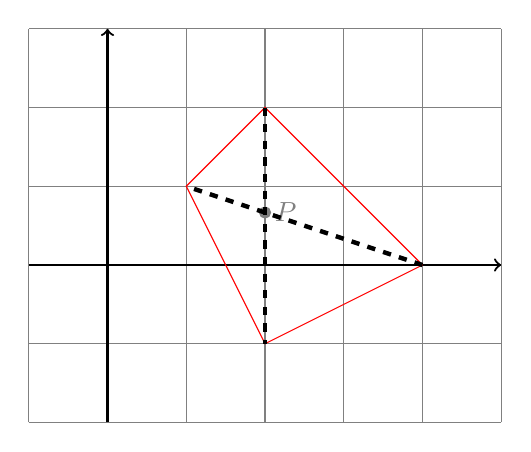
\begin{tikzpicture}[]
\draw [step=1.0,gray,thin] (-1,-2) grid (5,3);
\draw [thick,->](-1,0) -- (5,0); %x-axis
\draw [thick,->](0,-2) -- (0,3); %y-axis
\draw[red] (4,0) -- (2,2) -- (1,1) -- (2,-1) -- (4,0);
\filldraw [gray] (2,2/3) circle (2pt) node[right] {$P$};
\draw[black,dashed,ultra thick] (4,0) -- (1,1);
\draw[black,dashed,ultra thick] (2,2) -- (2,-1);
\end{tikzpicture}
\end{center}

Les dues rectes són:
\[
\begin{pmatrix}x\\y\end{pmatrix}=
\begin{pmatrix}1\\1\end{pmatrix}+\lambda
\begin{pmatrix}3\\-1\end{pmatrix}
\]
i
\[
\begin{pmatrix}x\\y\end{pmatrix}=
\begin{pmatrix}2\\2\end{pmatrix}+\mu
\begin{pmatrix}0\\-3\end{pmatrix}
\]
Igualant-les, obtenim les dues equacions:
\begin{eqnarray*}
  1+3\lambda &=& 2\\
  1-\lambda&=&2-3\mu
\end{eqnarray*}
De la primera obtenim que $\lambda=\frac{1}{3}$ que, substituït a la segona, ens diu que $\mu=\frac{4}{9}$. Substituint qualsevol d'aquests dos valors a les equacions paramètiques de les rectes obtenim que el punt buscat és  $P=(2,\frac{2}{3})$.

Les transformacions afins corresponents a les diferents operacions produeixen els canvis al quadrilàter mostrats a la Figura \ref{fig:trafquadril}.

  \begin{minipage}[t]{\linewidth}
    \vspace{-2ex}
    \includegraphics[width=\textwidth]{../figures/Afiquadrilater.pdf}
    \captionof{figure}{Transformacions afins d'un quadrilàter de vèrtex $(4,0)$, $(2,2)$, $(1,1)$ i $(2,-1)$.}
    \label{fig:trafquadril}
  \end{minipage}
